\documentclass[letterpaper,12pt]{article}
\usepackage[spanish, mexico]{babel}
\usepackage{siunitx}
\usepackage[utf8]{inputenc}
\usepackage{amsmath}
\usepackage{amssymb}
\usepackage{xcolor}
\usepackage[citecolor=blue]{hyperref}
\usepackage{fancyhdr}
\usepackage{listings}
\usepackage{newunicodechar}
\newunicodechar{́}{\'}
\usepackage[letterpaper, margin=1in]{geometry}
\usepackage{gensymb}
\usepackage{longtable}
\usepackage{booktabs}
\usepackage{tabularx}
\usepackage{colortbl}
\usepackage{parskip}
\usepackage[T1]{fontenc}
\usepackage{enumitem}
\usepackage{tikz}
\usetikzlibrary{arrows.meta,positioning,shapes.geometric}
\usepackage{graphicx}
\usepackage{float}
\usepackage{xurl}

\newcolumntype{C}{>{\centering\arraybackslash}X}

\hypersetup{
    colorlinks=true,
    linkcolor=black,
    filecolor=magenta,
    urlcolor=blue,
    citecolor=black
}

\definecolor{consolebg}{HTML}{1E1E1E}
\definecolor{consolefg}{HTML}{D4D4D4}
\definecolor{consolegreen}{HTML}{6A9955}
\definecolor{consoleyellow}{HTML}{DCDCAA}

\lstdefinestyle{pythonstyle}{
    language=Python,
    backgroundcolor=\color{white},
    basicstyle=\ttfamily\small,
    keywordstyle=\color{blue},
    stringstyle=\color{orange!80!black},
    commentstyle=\color{gray},
    breaklines=true,
    breakatwhitespace=true,
    numbers=left,
    numberstyle=\tiny\color{gray},
    frame=single,
    showstringspaces=false
}

\lstdefinestyle{consolestyle}{
    backgroundcolor=\color{consolebg},
    basicstyle=\ttfamily\footnotesize\color{consolefg},
    breaklines=true,
    breakatwhitespace=true,
    frame=single,
    framerule=0pt,
    rulecolor=\color{consolebg},
    xleftmargin=2pt,
    xrightmargin=2pt,
    showstringspaces=false
}

\setlength{\headheight}{76.27646pt}
\addtolength{\topmargin}{-34.27646pt}

\begin{document}

% --- PORTADA ---
\thispagestyle{empty}
\vspace*{-2.5cm}
\begin{center}
    \begin{tabularx}{\textwidth}{@{} l C r @{}}
    \raisebox{-0.5\height}{
\includegraphics[height=3.5cm]{image/izq.png}} &
    \parbox[c][3cm][c]{\linewidth}{\centering
        \Huge{\textbf{Universidad Nacional Autónoma de México}}\\[2pt]
        \LARGE{\textbf{Facultad de Ingeniería}}
    } &
    \raisebox{-0.5\height}{
\includegraphics[height=3.5cm]{image/der.png}}
    \end{tabularx}
\end{center}

\vspace{1cm}

\begin{center}
    \Huge{\textbf{Práctica 03\\}}
    \Huge{\textbf{\textit{Disco de Alberti}}}\\

    \vspace{1.5cm}
    \LARGE{\textbf{Asignatura:} }\\
    \vspace{0.2cm}
    \Large{Criptografía} \\
    \vspace{1cm}
    \LARGE{\textbf{Profesor:}}
    \LARGE{\textit{Dr. Alfonso Francisco De Abiega L'Eglisse}}\\
    \vspace{1cm}
    \Large{\textbf{Grupo:} 03} \\
    \vspace{1cm}
    \LARGE{\textbf{Integrantes - Equipo 10:} }\\
    \vspace{0.3cm}
    \Large{Espinoza Matamoros Percival Ulises} \\
    \Large{García Cortés Adolfo de Jesús} \\
    \Large{Lugo Manzano Rodrigo} \\
    \Large{Montiel Juárez Oscar Iván} \\
    \vspace{1cm}
    \Large{\textbf{Fecha de entrega:}}\\
    \vspace{0.2cm}
    \Large{{8 de Septiembre del 2026}}\\
    \vspace{1cm}
    \Large{\textbf{Semestre:} 2027-1}
\end{center}

\newpage

% --- CONFIGURACIÓN ENCABEZADO Y PIE ---
\pagestyle{fancy}
\fancyhf{}
\fancyhead[L]{
\includegraphics[width=1.5cm]{image/izq.png}}
\fancyhead[R]{
\includegraphics[width=1.5cm]{image/der.png}}
\fancyfoot[C]{\thepage}
\renewcommand{\footrulewidth}{0.4pt}
\pagenumbering{arabic}
\setcounter{page}{1}

\tableofcontents
\newpage

\begin{center}
{\LARGE \textbf{Práctica 03. Algoritmo de Cifrado: Disco de Alberti}}\\[0.5cm]
\end{center}

El disco de Alberti, ideado por Leon Battista Alberti en el siglo XV, es considerado el
antecesor de los cifrados polialfabéticos. A diferencia del cifrado César, en el que el
corrimiento entre el alfabeto plano y el cifrado permanece fijo durante todo el mensaje,
el disco de Alberti introduce un mecanismo mecánico: dos anillos concéntricos, uno fijo y
otro móvil, que pueden girarse entre sí para cambiar la correspondencia de letras a lo
largo del cifrado. Esto dificulta considerablemente el análisis de frecuencias, ya que una
misma letra del mensaje original puede cifrarse de distintas formas según el momento en que
se gira el disco.

\section{Explicación del Método}

El disco físico está compuesto por dos anillos con el alfabeto de 26 letras:

\begin{itemize}
    \item \textbf{Anillo fijo (exterior):} representa las letras del mensaje original, siempre
    en el mismo orden (\texttt{a, b, c, ..., z}).
    \item \textbf{Anillo móvil (interior):} representa las letras cifradas. Al girar el disco,
    el anillo móvil se desplaza, cambiando la letra con la que queda alineada cada posición
    del anillo fijo.
\end{itemize}

Antes de comenzar a cifrar, se define una \textbf{letra de alineación inicial}: es la letra
del anillo fijo con la que queda alineada la \texttt{a} del anillo móvil al arrancar. A partir
de ahí, el disco gira periódicamente conforme se van cifrando letras, usando dos parámetros:

\begin{itemize}
    \item \textbf{Periodo:} cada cuántas letras cifradas se gira el disco.
    \item \textbf{Paso:} cuántas posiciones avanza el anillo móvil cada vez que se gira.
\end{itemize}

Para cifrar una letra, se busca su posición en el anillo fijo y se toma la letra que le
corresponde en el anillo móvil, según el desplazamiento vigente. Cada vez que se cumple el
periodo, el desplazamiento aumenta en la cantidad indicada por el paso, simulando el giro
físico del disco. Los espacios en blanco se conservan tal cual y no cuentan como letras
cifradas, por lo que no provocan que el disco gire.

Para descifrar, el proceso se invierte: dada una letra cifrada, se busca su posición dentro
del anillo móvil (con el desplazamiento correspondiente) y se recupera la letra del anillo
fijo en esa misma posición. El desplazamiento se recalcula exactamente igual que en el
cifrado, por lo que ambas partes deben conocer la letra de alineación inicial, el periodo y
el paso para poder comunicarse correctamente.

\section{Implementación en Python}

El programa modela el anillo fijo como una cadena constante \texttt{A} con el abecedario, y
genera el anillo móvil de forma dinámica rotando dicha cadena según el desplazamiento
vigente.

\subsection{Generación del anillo móvil}

\begin{lstlisting}[style=pythonstyle]
A = "abcdefghijklmnopqrstuvwxyz"

def obtener_anillo_movil(desplazamiento):
    """
    Genera el anillo MOVIL (interior) del disco, rotado segun
    el desplazamiento actual. Simula "girar" fisicamente el disco.
    """
    return A[desplazamiento:] + A[:desplazamiento]
\end{lstlisting}

La rotación del anillo móvil se logra con una simple concatenación de rebanadas de la
cadena: la parte que queda "por delante" del corte se manda al final. Así, si el
desplazamiento es 3, el anillo móvil queda como \texttt{"defghijklmnopqrstuvwxyzabc"}, que
es justo lo que ocurriría si giráramos físicamente el disco tres posiciones.

\subsection{Función de cifrado}

\begin{lstlisting}[style=pythonstyle]
def cifrar(mensaje, letra_alineacion, periodo, paso, mostrar_detalle=False):
    mensaje_cifrado = ""
    desplazamiento = A.index(letra_alineacion)
    contador = 0

    for caracter in mensaje:
        if caracter in A:
            anillo_movil = obtener_anillo_movil(desplazamiento)
            indice = A.index(caracter)
            letra_cifrada = anillo_movil[indice]

            mensaje_cifrado += letra_cifrada
            contador += 1

            # Girar el disco cada 'periodo' letras cifradas
            if contador % periodo == 0:
                desplazamiento = (desplazamiento + paso) % len(A)
        else:
            # Los espacios se mantienen y NO giran el disco
            mensaje_cifrado += caracter

    return mensaje_cifrado
\end{lstlisting}

El desplazamiento inicial se obtiene ubicando la letra de alineación dentro del anillo fijo
\texttt{A}. Por cada letra válida que se cifra, se incrementa un contador independiente del
índice del mensaje, de forma que los espacios no alteran el conteo de letras para efectos
del giro. Cuando el contador alcanza un múltiplo del periodo, el desplazamiento avanza la
cantidad de posiciones indicada por el paso, tomando el módulo 26 para que el disco nunca
salga del rango del abecedario.

\subsection{Función de descifrado}

\begin{lstlisting}[style=pythonstyle]
def descifrar(mensaje_cifrado, letra_alineacion, periodo, paso, mostrar_detalle=False):
    mensaje_descifrado = ""
    desplazamiento = A.index(letra_alineacion)
    contador = 0

    for caracter in mensaje_cifrado:
        if caracter in A:
            anillo_movil = obtener_anillo_movil(desplazamiento)
            indice = anillo_movil.index(caracter)
            letra_original = A[indice]

            mensaje_descifrado += letra_original
            contador += 1

            if contador % periodo == 0:
                desplazamiento = (desplazamiento + paso) % len(A)
        else:
            mensaje_descifrado += caracter

    return mensaje_descifrado
\end{lstlisting}

El descifrado utiliza exactamente la misma lógica de giro que el cifrado —mismo
desplazamiento inicial, mismo periodo y mismo paso—, pero invierte la búsqueda: en lugar de
partir de la posición en el anillo fijo, se busca la letra cifrada dentro del anillo móvil
y se recupera la letra correspondiente del anillo fijo en esa posición. Al mantener
sincronizados ambos giros, el mensaje original se reconstruye letra por letra sin pérdida
de información.

\section{Pruebas del Programa}

Para validar el algoritmo se cifró el mensaje \textit{``hola equipo diez''} utilizando la
letra de alineación inicial \texttt{c}, un periodo de giro de \texttt{3} letras y un paso de
\texttt{5} posiciones. En la Figura~\ref{fig:cifrado} se muestra el detalle del cálculo para
cada letra durante el cifrado, incluyendo la letra con la que queda alineado el disco en el
momento de cifrar cada carácter.

\begin{figure}[H]
\centering
\begin{lstlisting}[style=consolestyle]
--- Calculo del cifrado (letra fija -> disco movil) ---
'h' (fijo pos  7) -> disco alineado en 'c' -> 'j'
'o' (fijo pos 14) -> disco alineado en 'c' -> 'q'
'l' (fijo pos 11) -> disco alineado en 'c' -> 'n'
'a' (fijo pos  0) -> disco alineado en 'h' -> 'h'
'e' (fijo pos  4) -> disco alineado en 'h' -> 'l'
'q' (fijo pos 16) -> disco alineado en 'h' -> 'x'
'u' (fijo pos 20) -> disco alineado en 'm' -> 'g'
'i' (fijo pos  8) -> disco alineado en 'm' -> 'u'
'p' (fijo pos 15) -> disco alineado en 'm' -> 'b'
'o' (fijo pos 14) -> disco alineado en 'r' -> 'f'
'd' (fijo pos  3) -> disco alineado en 'r' -> 'u'
'i' (fijo pos  8) -> disco alineado en 'r' -> 'z'
'e' (fijo pos  4) -> disco alineado en 'w' -> 'a'
'z' (fijo pos 25) -> disco alineado en 'w' -> 'v'
\end{lstlisting}
\caption{Cálculo del cifrado paso a paso, letra de alineación \texttt{c}, periodo 3, paso 5.}
\label{fig:cifrado}
\end{figure}

Puede observarse cómo el disco gira exactamente cada tres letras cifradas: se mantiene
alineado en \texttt{c} para las primeras tres letras, luego pasa a \texttt{h} (avanzando 5
posiciones), después a \texttt{m}, a \texttt{r} y finalmente a \texttt{w}. Los espacios en
blanco del mensaje no aparecen en el detalle porque se copian directamente sin consumir un
giro del disco.

En la Figura~\ref{fig:descifrado} se muestra el proceso inverso, junto con el bloque de
resultados finales que confirma que el mensaje descifrado coincide exactamente con el
mensaje original.

\begin{figure}[H]
\centering
\begin{lstlisting}[style=consolestyle]
--- Calculo del descifrado (disco movil -> letra fija) ---
'j' (movil alineado en 'c') -> pos  7 -> 'h'
'q' (movil alineado en 'c') -> pos 14 -> 'o'
'n' (movil alineado en 'c') -> pos 11 -> 'l'
'h' (movil alineado en 'h') -> pos  0 -> 'a'
'l' (movil alineado en 'h') -> pos  4 -> 'e'
'x' (movil alineado en 'h') -> pos 16 -> 'q'
'g' (movil alineado en 'm') -> pos 20 -> 'u'
'u' (movil alineado en 'm') -> pos  8 -> 'i'
'b' (movil alineado en 'm') -> pos 15 -> 'p'
'f' (movil alineado en 'r') -> pos 14 -> 'o'
'u' (movil alineado en 'r') -> pos  3 -> 'd'
'z' (movil alineado en 'r') -> pos  8 -> 'i'
'a' (movil alineado en 'w') -> pos  4 -> 'e'
'v' (movil alineado en 'w') -> pos 25 -> 'z'

------------- Resultados -------------

--> Letra de alineacion inicial:  c
--> Periodo de giro:               3
--> Paso de giro:                  5
--> Mensaje original:              hola equipo diez
--> Mensaje cifrado:               jqnh lxgubf uzav
--> Mensaje descifrado:            hola equipo diez
\end{lstlisting}
\caption{Cálculo del descifrado y verificación del resultado final.}
\label{fig:descifrado}
\end{figure}

El mensaje \textit{``hola equipo diez''} se cifra como \textit{``jqnh lxgubf uzav''}, y al
aplicar el descifrado con los mismos parámetros se recupera exactamente el mensaje original,
lo que confirma que el giro del disco se mantiene sincronizado en ambas direcciones.

La Figura~\ref{fig:ejecucion-completa} presenta la ejecución completa del programa. En ella
se verifican los parámetros de entrada, el mensaje cifrado y la recuperación correcta del
mensaje original al aplicar el descifrado.

\begin{figure}[H]
\centering
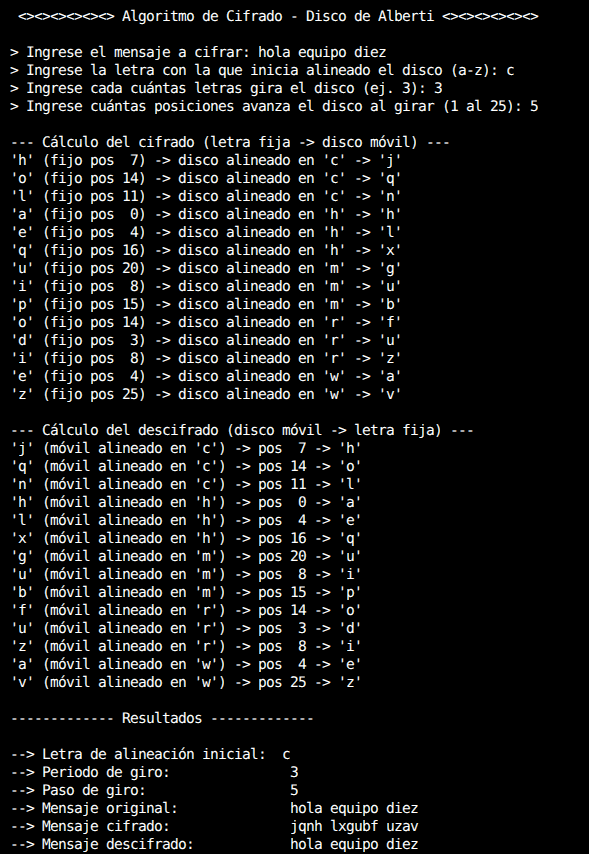
\includegraphics[width=0.85\textwidth]{image/ejecucion_1.png}
\caption{Prueba de ejecución completa del programa del disco de Alberti.}
\label{fig:ejecucion-completa}
\end{figure}

\section{Repositorio}

El código correspondiente a esta práctica 3 se puede consultar en el siguiente repositorio:

\url{https://github.com/percivalespi/Criptografia/blob/main/practica3/codigo/disco_alberti.py}

\section{Conclusión}

Implementar el disco de Alberti nos permitió entender de forma práctica por qué se le
considera el punto de partida de los cifrados polialfabéticos: a diferencia del César y del
Vigenère, aquí el corrimiento no depende de una palabra clave letra por letra, sino de un
mecanismo de giro periódico que puede ajustarse en frecuencia (periodo) e intensidad (paso).
El reto principal fue separar correctamente el conteo de letras cifradas del recorrido del
mensaje completo, de modo que los espacios no interfirieran con el momento exacto en que el
disco debía girar. Usar el operador módulo sobre la longitud del alfabeto, junto con una
variable de contador independiente, nos permitió simular de forma fiel el comportamiento
físico del disco y comprobar que el cifrado y el descifrado permanecen perfectamente
sincronizados.

\end{document}
